The concept of performance assessment of the service delivery of aggregators was presented by one of this work's authors in \cite{bondy2014performance}, but inconsistencies and shortcomings have been found in the proposed assessment index. Based upon work presented in \cite{thavlov2015thesis}, the service performance assessment index is corrected and expanded upon here. In order to asses service performance three concepts are introduced in this section:
\begin{itemize}
\item Quality of service, which is an instantaneous measure of how well the aggregator is delivering one service within the contract constraints;
\item service performance assessment index, which describes the overall performance of the aggregator over the delivery period for the services, or subset of services, it is providing; and a
\item service verification index, which describes how much an aggregator is breaking the contractual agreements (non-delivering) of the services, or a subset of services, it provides.
\end{itemize}

Differently from the previous work, the service delivery index is split into measures of the ancillary services (AS) delivered to system operators and the AMS delivered to unit owners (see Sec.~\ref{sec:DERs}). In this way, a system operator (or a third party certification company) can use the index for certification of aggregators, for which the AMS evaluation is irrelevant. Furthermore, the service verification index is introduced, and a new way of defining the quality of service is presented.
%\athanote{We should be a bit more explicit about services delivered upwards in the system (AS) and down-wards (AMS) to the asset owner}

\subsection{Quality of Service}
Quality of service (QoS) is a measure defined in \cite{bondy2014performance}, where it is used to assess the quality of a power system service at any given time. QoS at any given time is given by:
\begin{equation}\label{eq:QoS}
QoS(t)=e(t)C_{s}(t)
\end{equation}
where \emph{e(t)} is the error in service delivery introduced in Sec.~\ref{sec:SEGANmethodology}, and $C_s(t)$ is a normalization factor that can be time varying. By definition:
\begin{itemize}
\item $QoS \geq 0$;
\item for $QoS \leq 1$ the service is considered delivered within the contractual constraints;
\item and $QoS = 0$ is a perfect service delivery.
\end{itemize}
In order to achieve these definitions, the normalization factor $C_{s}(t)$ must be calculated from $\mathbf{x}_{acc}(t)$ thus:
\begin{equation}
C_{s}(t) = 
\begin{cases}
\frac{1}{x_{acc,max}(t) - x_{max}(t)}, & e(t) \geq 0 \\
\frac{1}{x_{acc,min}(t) - x_{min}(t)}, & e(t) < 0.
\end{cases}\label{eq:cst}
\end{equation}
where $x_{acc,max/min}$ and $x_{max/min}$ are part of the service model defined in Sec.~\ref{sec:SEGANmethodology}. By defining $C_{s}(t)$ in this way, we take into account the possibility of asymmetry in the values of $x_{acc}$, and ensure that QoS is a positive value. A visual representation of this scaling can be seen in Fig.~\ref{fig:tracking_error}--Fig.~\ref{fig:cap_error}, where the QoS for the three kinds of services are presented.
In general, the rate with which $QoS(t)$ increases depends on the difference between $x_{acc}(t)$ and $x_{ideal}(t)$.
\begin{figure}
\centering
\subfloat[Error]{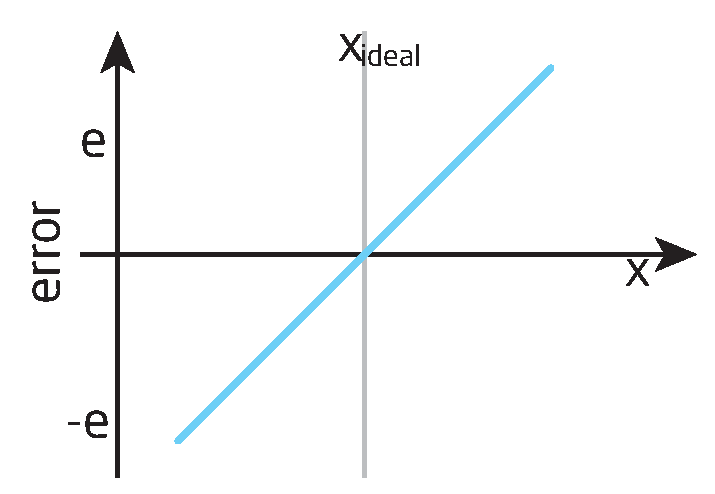
\includegraphics[width=0.5\columnwidth]{SEGAN/tracking_error2.eps}%
\label{fig:errortracking}} \subfloat[Quality of Service]{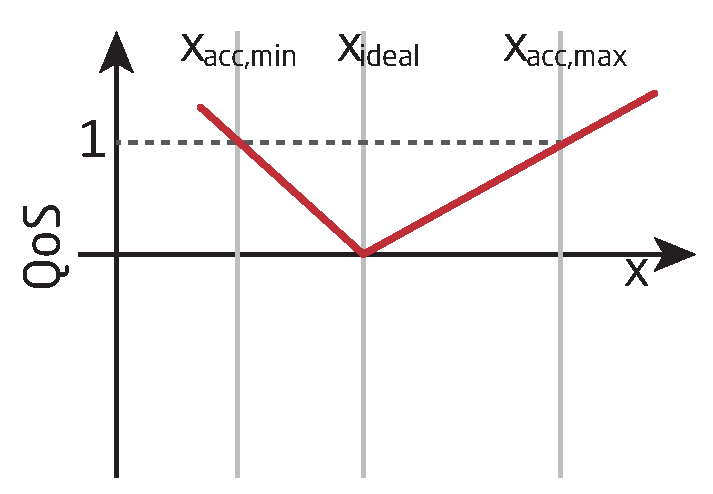
\includegraphics[width=0.5\columnwidth]{SEGAN/tracking_error3.eps}%
\label{fig:qostracking}}
\caption{Error and QoS for tracking services, note that the acceptable band do not need to be symmetric.}
\label{fig:tracking_error}
\end{figure}
\begin{figure}
\centering
\subfloat[Error]{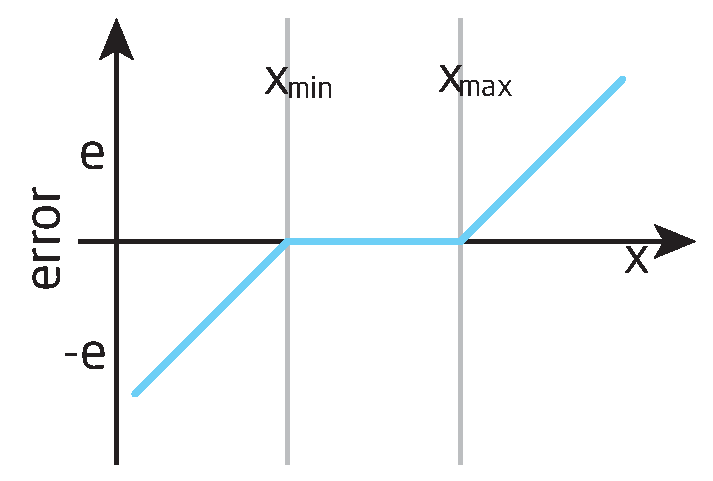
\includegraphics[width=0.5\columnwidth]{SEGAN/band_error2.eps}%
\label{fig:errorband}}\subfloat[Quality of Service]{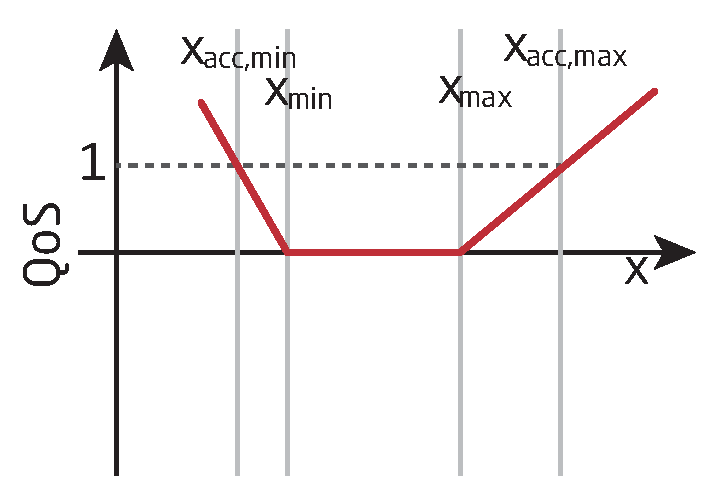
\includegraphics[width=0.5\columnwidth]{SEGAN/band_error3.eps}%
\label{fig:qosband}}
\caption{Error and QoS for band services.}
\label{fig:band_error}
\end{figure}
\begin{figure}
\centering
\subfloat[Error]{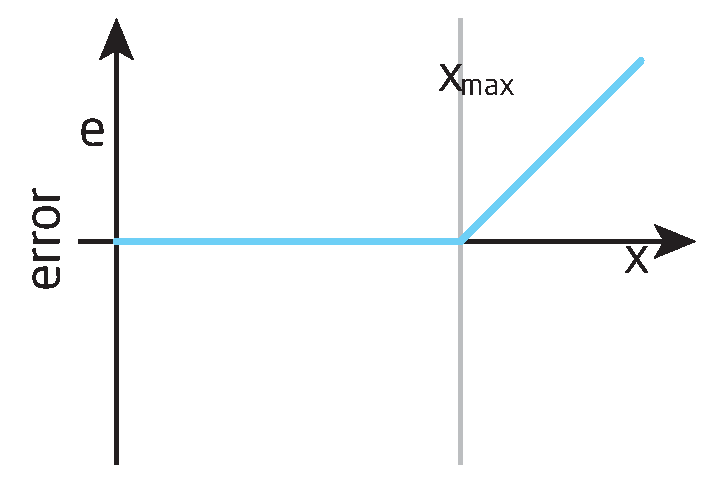
\includegraphics[width=0.5\columnwidth]{SEGAN/cap_error2.eps}%
\label{fig:errorcap}}
\subfloat[Quality of Service]{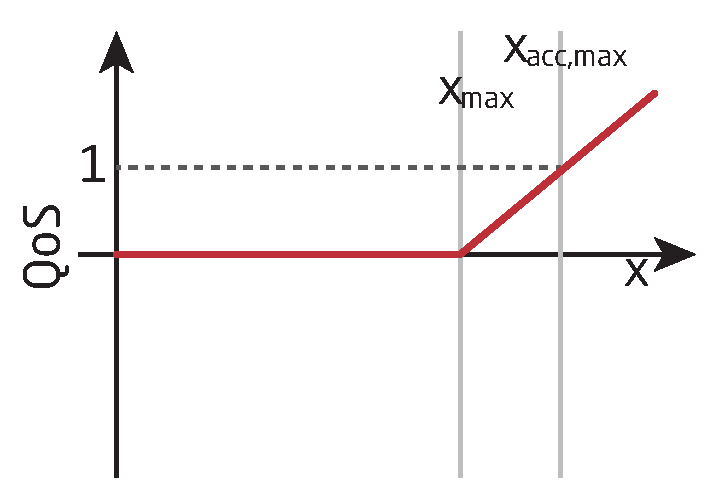
\includegraphics[width=0.5\columnwidth]{SEGAN/cap_error3.eps}%
\label{fig:qoscap}}
\caption{QoS for a maximum cap service, a minimum cap service is defined similarly but with $x_{min}$ and $x_{acc,min}$ values.}
\label{fig:cap_error}
\end{figure}
%\begin{figure*}[!t]
%\centerline{\subfloat[Case I]\includegraphics[width=2.5in]{subfigcase1}%
%\label{fig_first_case}}
%\hfil
%\subfloat[Case II]{\includegraphics[width=2.5in]{subfigcase2}%
%\label{fig_second_case}}}
%\caption{Simulation results}
%\label{fig_sim}
%\end{figure*}

Note that in \eqref{eq:cst}, $C_{s}(t)$ is not defined for $x_{acc}(t) = x_{ideal}(t)$. This is a corner case, in which:
%\bondynote{This QoS is only used then to calculate the Non-Delivery K, so, since we subtract 1 later on anyway, we might as well say the cornercase automatically starts counting on the Non-Delivery, and QoS = 1 for $e \neq 0$}
\begin{equation}
QoS(t) = e(t), \quad x_{acc}(t) = x_{ideal}(t)
\end{equation}


\subsection{Assessing service delivery}
Having defined an instantaneous measure for the quality of individual services, we can evaluate the aggregator as a whole based upon the quality of all the services it delivers. The chosen requirements for such and index are \cite{bondy2014performance}:
\begin{itemize}
	\item[R1] Provide a \emph{quality} measure normalized to the contractual requirements (bounds) of a service. 
	\item[R2] The measure should be normalized with respect to time.
	\item[R3] Provide a \emph{reliability} measure in relation to service non-delivery.
	\item[R4] Each service must have a separate, individually verifiable, measure. For example, to evaluate service delivery w.r.t. ancillary-service delivery, the asset-management quality is irrelevant.
\end{itemize}

The overall service delivery index of AS is defined by $\eta^{AS}$ in Eq.~\eqref{eq:etaAS}, but before calculating the index the QoS must be cleaned. To sort out non-delivery incidents (which are measured apart), we clamp $QoS_{K,meas}^{AS}(t)$ (the measured quality of service for the \emph{K} ancillary services the aggregator is providing) such that it does not account for $QoS \geq 1$: 
\begin{algorithmic}[H]
\FOR{ t = 0:$t_N$ }
\FOR{ i = 1:K}
    \IF{$QoS_{i,meas}^{AS}(t)>1$} 
        \STATE $QoS_{i}^{AS}(t) = 1$ 
    \ELSE 
        \STATE $QoS_{i}^{AS}(t) = QoS_{i,meas}^{AS}(t)$
    \ENDIF
\ENDFOR
\ENDFOR
\end{algorithmic}
where \emph{K} is the total number of AS the aggregator provide.
This clamping is not done in \cite{bondy2014performance} since that work did not use of a separate non-delivery index. This means that $\eta_{AS}$ is only a measure of the service provision performance within the contractual limits.

While the previous definitions have been established in continuous time, the actual measurement and calculations are done in discrete time. This leads to $\eta_{AS}$ being estimated for \emph{K} amount of AS over each corresponding discrete time horizon $N_K$:
\begin{align}\label{eq:etaAS}
\eta^{AS} &= \sum^{K}_{i=1} W_i \sqrt{\frac{\sum^{N_i}_{t=0} \left( {QoS^{AS}_{i,t}}^{2} \right)}{N_i}}\\
\sum_{i=1}^K W_i &= 1
\end{align}
where $W_K$ is the assigned weight to each AS, leading to $\eta^{AS} \in [0,1]$, and $\eta$ close to zero representing good performance while $\eta$ close to 1 representing a barely acceptable performance. This means that the service performance assessment index for all the AS the aggregator provides is a weighted average of the root mean square (RMS) of the error in all service deliveries. With this index it is possible to evaluate aggregators that deliver more than one AS at a time, e.g. a frequency containment reserve and a replacement reserve, and assign a hierarchy of importance with respect to the services. However, how to do distinguish measurements to verify the services, and how to evaluate which service is more important, is out of scope of this work, but the definition of Eq.~\eqref{eq:etaAS} takes the possibilities into account. In the case where only a single service delivery is considered, Eq.~\eqref{eq:etaAS} is simply the RMS of the error in service delivery:
\begin{equation}\label{eq:etaASsimp}
\eta^{AS} = \sqrt{\frac{\sum^{N}_{t=0} \left( {QoS^{AS}_{t}}^{2} \right)}{N}}.
\end{equation}

Similarly, the ability of the aggregator to deliver AMS as a whole can be measured with an index $\eta^{AMS}$ (Eq.~\eqref{eq:etaAMS}). In this instance, QoS is also clamped to $QoS^{AMS}_{M}(t) \in [0,1]$, and the amount of \emph{M} services are evaluated for their corresponding time horizon $N_M$:
\begin{equation}\label{eq:etaAMS}
\eta^{AMS} = \sum^{M}_{i=1} W_i \sqrt{\frac{\sum^{N_i}_{t=0} \left( {QoS^{AMS}_{i,t}}^{2} \right)}{N_i}}
\end{equation}
with $\eta^{AMS} \in [0,1]$. Each of these indices give an idea of the performance of the aggregator where the duration of time delivery is taken into account. This means that two service provisions are evaluated equally when their error in service delivery compared to the duration of the service delivery are the same. With these definitions, requirements \emph{R1}, \emph{R2} and \emph{R4} are fulfilled.

Finally, if the aggregator desires to have an internal overall evaluation of all the services it is providing, it can do so through a weighted mean of the service performance indices:
\begin{equation}
\eta_{tot} = \alpha \eta^{AS} + (1-\alpha) \eta^{AMS}, \quad \alpha \in [0,1]
\end{equation}
where $\alpha$ is the weight ratio the aggregator assigns to the performance of the services.

\subsection{Verifying service delivery}
Requirement \emph{R3} mentioned in the previous section asks for a reliability measure. To address this requirement, an index $\epsilon^{AS}$, similar to the service performance assessment index, is defined for verifying the delivery of AS\footnote{This can also be interpreted as evaluating non-delivery of service.} and an index $\epsilon^{AMS}$ is defined for the verification of AMS. Also, a non-delivery measure for the AS provision, $ND^{AS}$, is defined according to the following pseudo code:

\begin{algorithmic}[H]
\FOR{ t = 0:$t_N $}
\FOR{ i = 0:K}
    \IF{$QoS^{AS}_{i,meas}(t)<1$} 
        \STATE $ND^{AS}(t) = 0$ 
    \ELSE 
        \STATE $ND^{AS}(t) = QoS^{AS}_{i,meas}(t)-1$
    \ENDIF
\ENDFOR
\ENDFOR
\end{algorithmic}
This clamping shows that whenever the QoS of a service exceeds 1, i.e. the limit of what is an acceptable service provision, the amount with which it breaks the acceptable constraint is measured by \emph{ND}.
$\epsilon^{AS}$ is calculated in the same way as $\eta^{AS}$ using $ND^{AS}_K(t)$ instead of $QoS^{AS}_{K}(t)$:

\begin{equation}\label{eq:epsilonAS}
\epsilon^{AS} = \sum^{K}_{i=1} W_i \sqrt{\frac{\sum^{N_i}_{t=0} \left( {ND^{AS}_{i,t}}^{2} \right)}{N_i}}
\end{equation}
where $\epsilon^{AS} \in [0,\infty]$.

The same clamping process is applied to the non-delivery measure of the AMS, and $\epsilon^{AMS}$ is defined as:
\begin{equation}\label{eq:epsilonAMS}
\epsilon^{AMS} = \sum^{M}_{i=1} W_i \sqrt{\frac{\sum^{N_i}_{t=0} \left( {ND^{AMS}_{i,t}}^{2} \right)}{N_i}}.
\end{equation}

Thus $\epsilon$ is used to asses the severity of non-delivery events. For some systems it is critically important that $QoS(t)\leq1$ at any time, in which case $\epsilon$ should be close to zero for the contract to be considered respected. Other systems can tolerate $QoS(t)>1$ for some period, which leads to a higher acceptable $\epsilon$. A service delivery is verified if $\epsilon \leq \epsilon_{max}$, and this contractual limit, i.e. the value of $\epsilon_{max}$, must be assessed individually depending on the nature of the system. It is likely that in most cases $\epsilon^{AS}_{max}<\epsilon^{AMS}_{max}$, since the security of the power system is more important than, e.g., the temperature comfort of a home owner.

In \cite{bondy2014performance}, non-delivery is assesed using a non-delivery counter (NDC). $\epsilon$ differs from the NDC in that it both captures the time span of non-delivery and the magnitude of the violation, whereas NDC only captures the amount of time samples where non-delivery is detected. $\epsilon$ might prove advantageous over the NDC as a service verification index for some systems. A disadvantage of $\epsilon$ is that it might be a less intuitive measure to communicate to the service providers compared to the NDC.

Fig. \ref{fig:RefErr} shows an example of reference tracking error service performance assessment. Deviations between $x_{act}$ and $x_{ideal}$ inside the band defined by $x_{acc}$ will lead to $QoS<1$, while deviations outside the $x_{acc}$ band will lead to $QoS>1$. For this particular example $\eta^{AS}=0.7501$ and the service verification index is $\epsilon^{AS}=0.2324$, which indicates that generally the service provision is bad at following the reference, and also has a moderate amount of non-delivery. The service acquirer will have to decide whether this verification index value is acceptable or if it should lead to economical penalization or contract termination.

\begin{figure}
\centering
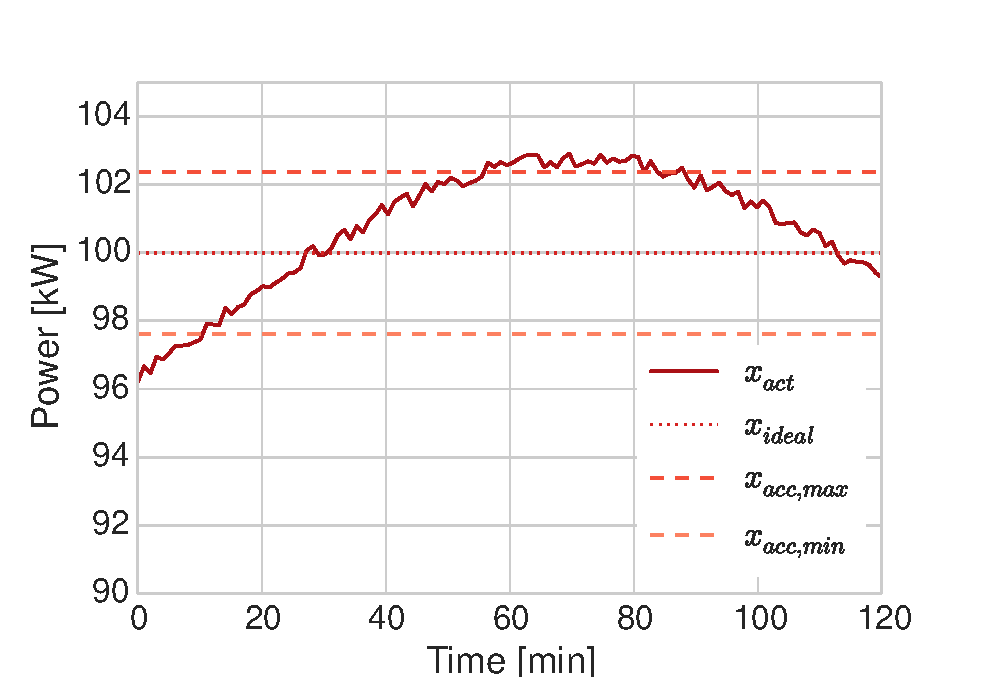
\includegraphics[width=\columnwidth]{SEGAN/reftrack.eps}
\caption{Example of reference tracking error with performance $x_{act}$, ideal performance $x_{ideal}$ and tolerance limits $x_{acc}$.}
\label{fig:RefErr}
\end{figure}
